\begin{center}
	\begin{abstract}
		This is the design document of Chaitanya Sharma for Project 3 for ECE 250's Winter 2023 offering.
	\end{abstract}
\end{center}

\section{Introduction}
My program consists of a major class {\color{draculapurple}Trie}, and two nested classes inside that ,namely {\color{draculapurple}Node} and
	{\color{draculapurple}NASIS}.
	While the {\color{draculapurple}Trie} class is an aggregate of the {\color{draculapurple}Node} class, the {\color{draculapurple}NASIS} class is a helper {\textbf{information}} class which allows me to create a single search function for insertion and deletion of nodes.
Also, I've created a {\color{draculayellow}trietest.cpp} file to contain the driver code which runs a while loop to parse inputs. There is also an excetion class called {\color{draculapurple}IllegalException} which I've inherited from the {\color{draculapurple}std::exception} class.
I attribute the latex template which I've used for this design document to myself as I've used it in the past for my other projects in this course.
\newline I've tested all edge test cases possible and also used the test cases provided by the
jekelautograder on {\color{DarkPastelBlue}https://github.com/JZJisawesome/ece250-testcases}.
\newline
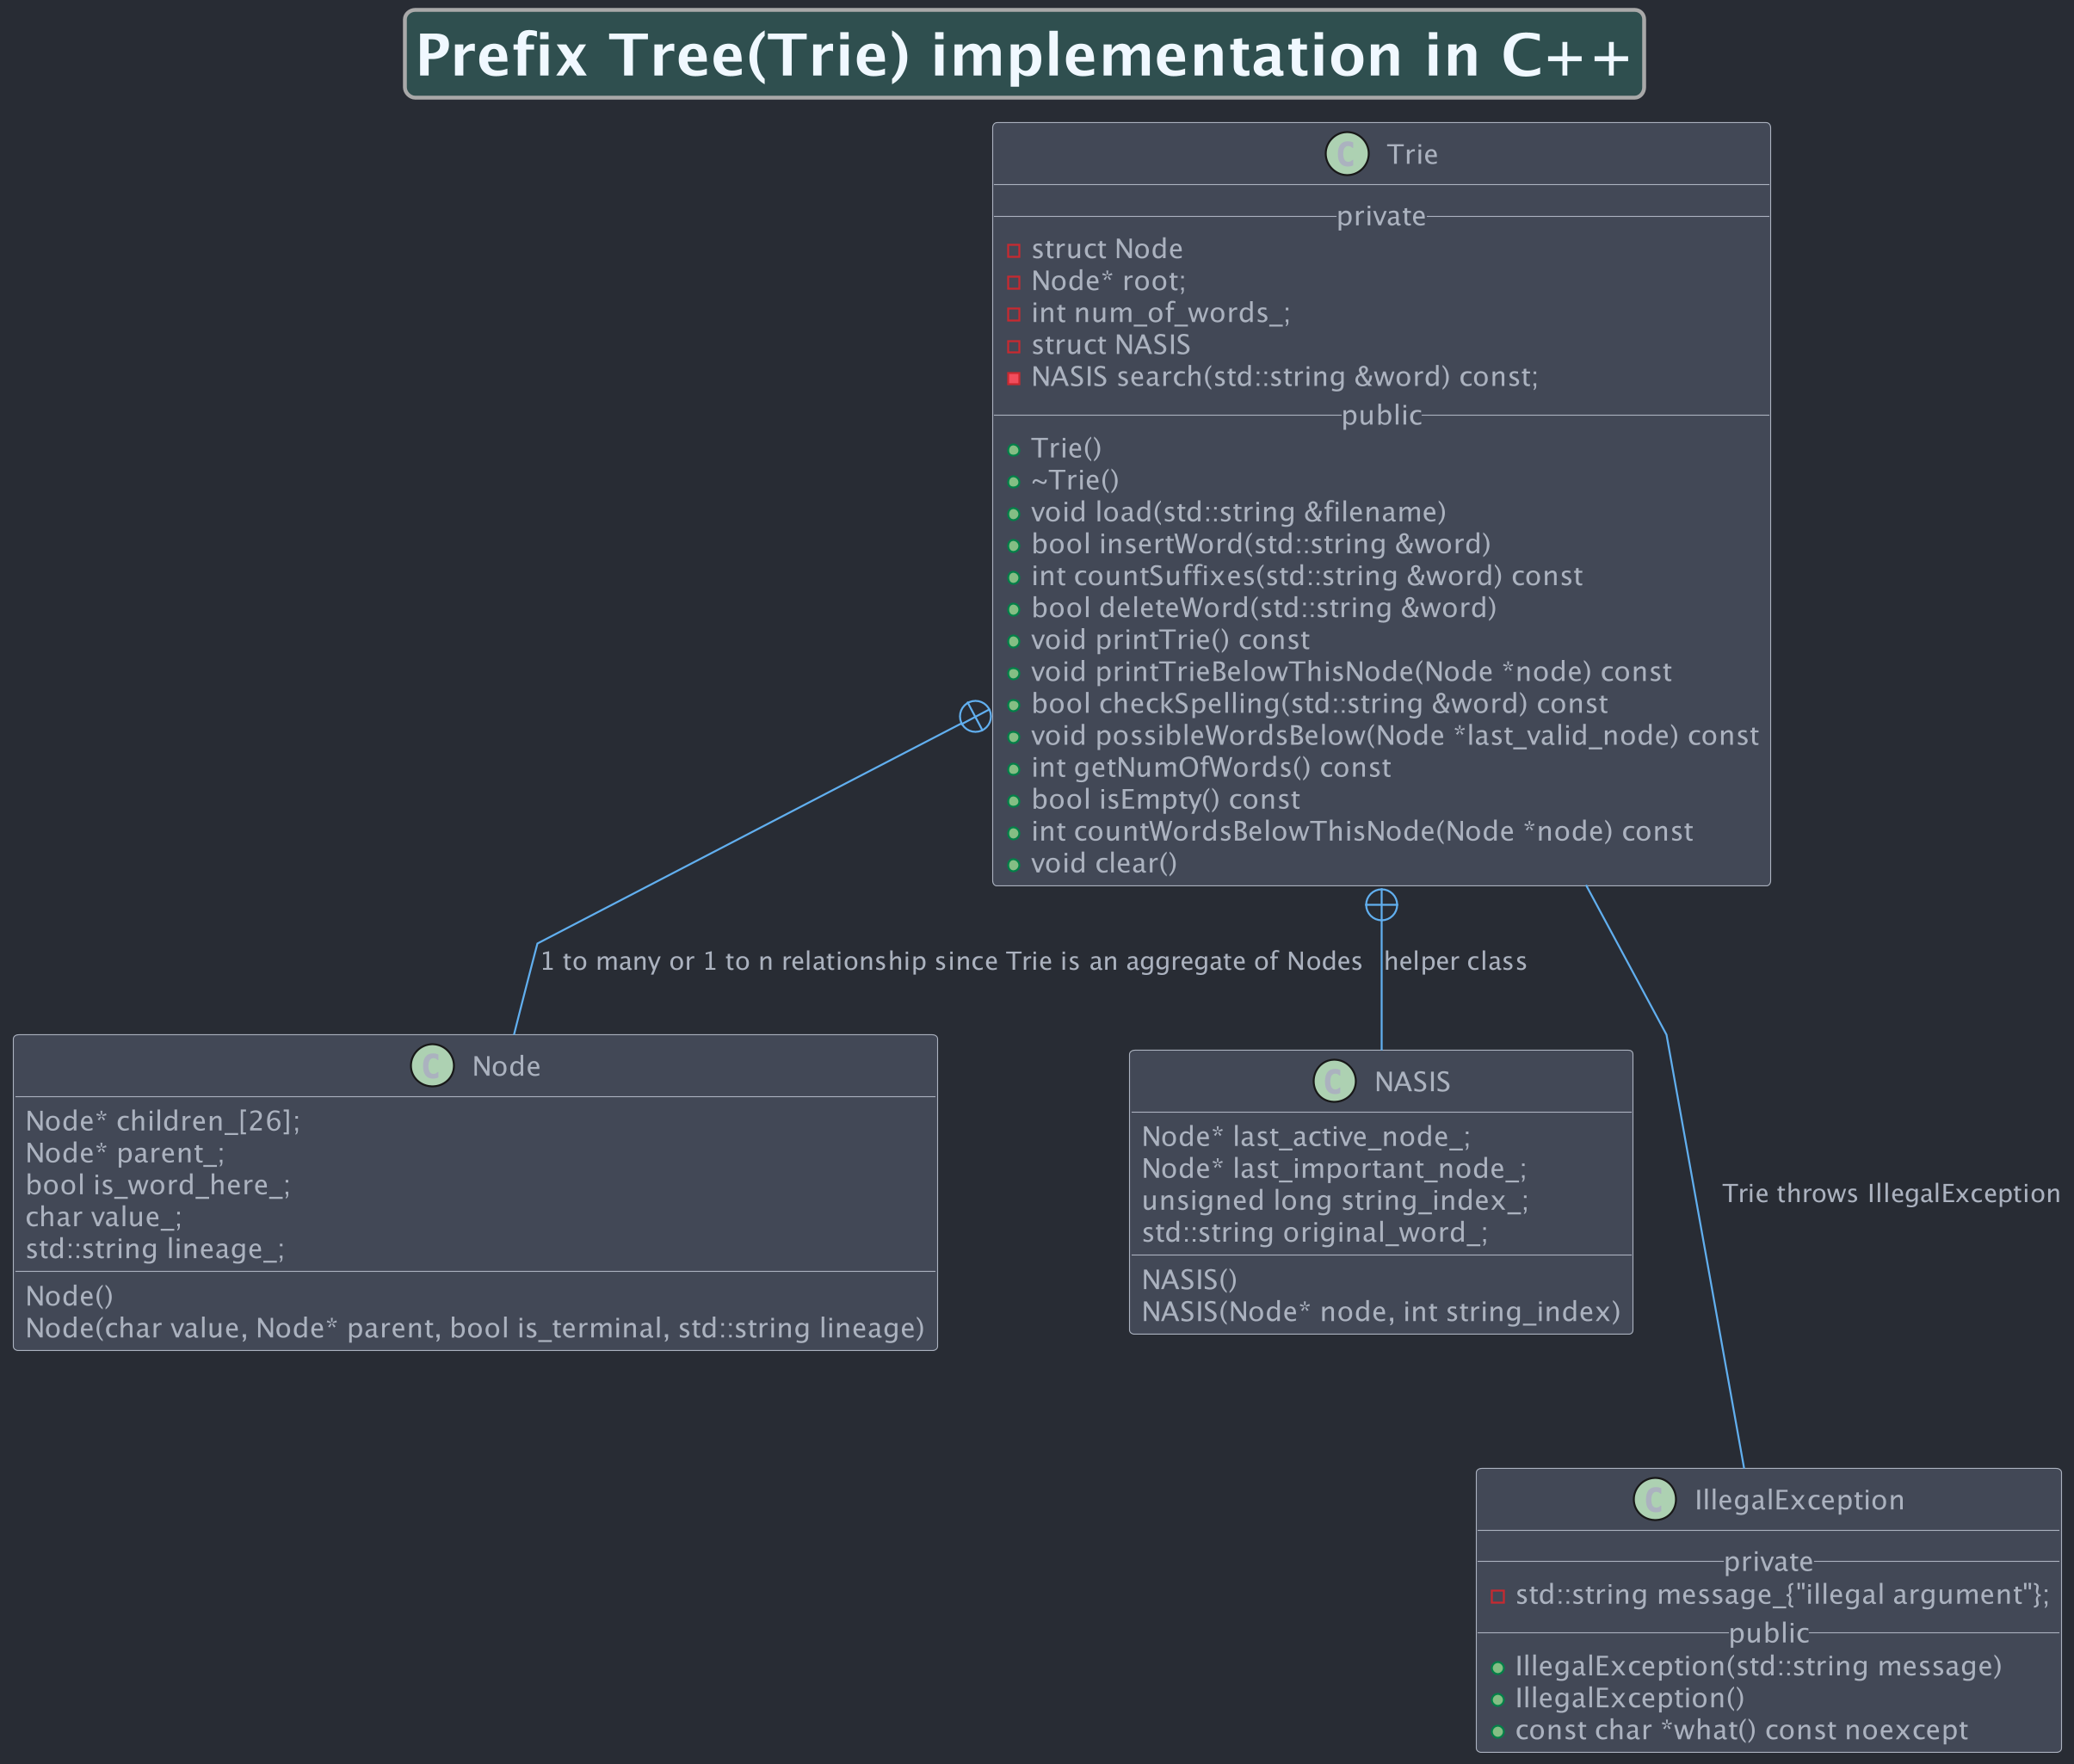
\includegraphics[scale=0.145, center]{PrefixTrie.png}
\section{Class Structure}



\subsection{{\color{orange}class} {\Large{\color{draculapurple}IllegalException}}}
I'm using a default constructor and a parameterized constructor for this class. Though I'm not using the parameterized constructor in my code, I've included it for future use.
This is a simple exception class which I've inherited from the {\color{draculapurple}std::exception} class. 
It has a private member variable {\color{Turquoise}message\_} which is a string which stores the message to be 
displayed when the exception is thrown. It has a constructor which takes a string as an argument and assigns it 
to the {\color{Turquoise}message\_} variable. It also has a default constructor which assigns the default 
message to the {\color{Turquoise}message\_} variable. It has a {\color{draculapurple}what()} function which returns 
the {\color{Turquoise}message\_} variable as a {\color{draculapurple}const char*}.

\subsection{{\color{orange}class} {\Large{\color{draculapurple}Trie}}}
The {\color{draculapurple}constructor} for this class just initializes the {\color{draculapurple}root\_} pointer and the {\color{draculapurple}num\_of\_words\_} variable to 
{\color{draculapurple}nullptr} and {\color{draculapurple}0} respectively. The {\color{draculapurple}destructor} for this class just deletes the {\color{draculapurple}root\_} pointer, which indirectly deletes all the nodes in the trie.
This is the major and the only top level class in my whole code. The most important member object of this class is a {\color{draculapurple}root\_} of 
type {\color{draculapurple}Node} which is a pointer to the root node of the trie. And the only other member object is a {\color{draculapurple}num\_of\_words\_} 
which is an integer which stores the number of words in the trie.

\subsubsection{{\color{orange}class} {\color{draculapurple}Node} (private nested class)}
This is a private nested class inside {\color{draculapurple}Trie} class. A simple class which has a static array of 26 pointers to other nodes i.e. its {\color{Turquoise}children}, initialized to nullptr, has a {\color{Turquoise}parent} pointer, 
an inherent {\color{Turquoise}character value}, a {\color{Turquoise}lineage} which contains a string of all nodes from root node to itself, and a boolean variable which 
tells whether the node is a {\color{Turquoise}word ending} node or not.
It's {\color{draculapurple}destructor} is created such that it deletes all the nodes which are children of itself, and then deletes itself.

\subsubsection{{\color{orange}class} {\color{draculapurple}NASIS} (stands for {\color{draculapurple}N}ode {\color{draculapurple}A}nd {\color{draculapurple}S}tring {\color{draculapurple}I}ndex for {\color{draculapurple}S}earching)  (private nested class)\newline
\faStar~~{\color{Awesome}a special feature of my code}~~\faStar}
This is a quintessential but convenient helper class which I've created to help me with the search function. 
It has 4 member objects, namely {\color{draculapurple}last\_active\_node\_}, {\color{draculapurple}last\_important\_node\_}, {\color{draculapurple}string\_index\_} and {\color{draculapurple}original\_word\_}.	
The reason I implemented this is because traversal in trees is extremely common, as well as expensive, hence it should make sense to make a single function for traversing the prefix trie, 
I had the same idea for the Linked List project as well as for the Hash Table Project, but they were both linear structures(in the sense of the base structure), but this project is not, 
hence we need more information to be returned, since I would always use a word to find the appropriate node for mutation and accession, I have the string index, which returns the 
character at the last valid node when traversing in the path of the word. {\color{draculapurple}last\_important\_node\_} which either has more than one child, 
or is a word ending node before traversing to the possible {\color{draculapurple}last\_active\_node\_}, which is the last possible node with the same 
{\color{draculapurple}lineage\_} as the word, and the {\color{draculapurple}original\_word\_} which is the word itself. 
More info in the search function subsubsection. 



\subsubsection{{\color{orange}NASIS} {\color{draculapurple}search}({\color{orange} std::string} word) {\color{GoldenYellow} const}}
This function is aimed at reducing redundant traversals in my code, and handles the search for a word operation in the Trie. 
It takes in a {\color{orange}std::string} word, and from the root, traverses the trie parallel to what character appears in an increasing index value in the word.
Along the way, if it observes any node with more than one child, or a word ending node, it rewrites the pointer node in {\color{draculapurple}last\_important\_node\_}. 
If it sees that there is no child node for the current character, it returns the {\color{draculapurple}NASIS} object with the {\color{draculapurple}last\_active\_node\_} 
as the last node which has the same {\color{draculapurple}lineage\_} as the word, and the {\color{draculapurple}string\_index\_} as the index of the last character 
in the word which is valid. The information aims to make a single function for traversing the trie, and then using the information to perform the required operation.
This function runs in {\color{lightblue}O(n)} where {\color{lightblue}n} is the number of characters in the word.

\subsubsection{{\color{orange}void} {\color{draculapurple}load}({\color{orange} std::string} filename)}
This function uses the C++ standard library {\color{orange}std::ifstream} class to read the file and load the words into the trie using the {\color{draculapurple}insert} function repeatedly on the appearing words.
This function outputs {\color{green}success} no matter what. This function runs in {\color{lightblue}O(n)} where {\color{lightblue}N} where N is the number of words in the file 
though it is directly dependant on the number of words, but since it callse the {\color{draculapurple}insert} function which runs in {\color{lightblue}O(n)} where {\color{lightblue}n} 
is the number of characters in the word, the time complexity is the same.
{\color{GoldenYellow} "load"}

\subsubsection{{\color{orange}bool} {\color{draculapurple}insert}({\color{orange} std::string} word)}
This function inserts a word into the trie, it uses the {\color{draculapurple}search} function to get the appropriate information from the NASIS object, 
then, if the {\color{draculapurple}string\_index\_} is equal to the length of the word, it checks if the {\color{draculapurple}last\_active\_node\_} 
is a word ending node, if it is, it returns false, otherwise, it sets the {\color{draculapurple}is\_word\_here\_} boolean to true, and increments the 
number of words in the trie, and returns true. If the {\color{draculapurple}string\_index\_} is not equal to the length of the word, it gets the substring
 of the word from the {\color{draculapurple}string\_index\_} to the end, and then traverses the trie from the {\color{draculapurple}last\_active\_node\_} 
 and creates new nodes for each character in the substring, and then sets the {\color{draculapurple}is\_word\_here\_} boolean to true, and increments the
  number of words in the trie, and returns true. This function runs in {\color{lightblue}O(n)} where {\color{lightblue}n} is the number of characters in the word.
  Also, this function, if comes across a character outside the range of capital english alphabets, it throws an exception of type {\color{orange}IllegalException}.
  {\color{GoldenYellow} "i"}


\subsubsection{{\color{orange}int} {\color{draculapurple}countSuffixes}({\color{orange} std::string} word) {\color{GoldenYellow} const} And {\color{orange}int} {\color{draculapurple}countWordsBelowThisNode}({\color{orange} Node} *node) {\color{GoldenYellow} const}}
The function {\color{draculapurple}countSuffixes}  counts the number of suffixes of a word in the trie, first it traverses the trie parallel to the word, and if it 
finds a node with no child for the current character, it returns false. Otherwise it completes the loop, and then uses the 
{\color{draculapurple}countWordsBelowThisNode} function to count the number of words below the last active node, which is the 
last node with the same lineage as the word. This function runs in {\color{lightblue}O(N)} where {\color{lightblue}N} is the 
number of characters in the word. The reason this function runs in {\color{lightblue}O(N)} and not {\color{lightblue}O(n)} (where n is the number of characters in the word) is because the average word in the English language has between 4-7 characters, and even if we assume that the word has 1000 characters, which situation is very unlikely, {\color{lightblue}O(1000N)} is still {\color{lightblue}O(N)}. Also, it can be safely assumed that M, the maximum characters in a word, $M<<N$ and that the number of characters in the trie are a constant multiple of the number of words.
The function {\color{draculapurple}countWordsBelowThisNode} counts the number of words below a node, it uses recursion to traverse the trie, and if it finds a word ending node, it increments the count, and then returns the count. This function runs in {\color{lightblue}O(N)} where {\color{lightblue}N} is the number of words in the trie.
Also, this function, if comes across a character outside the range of capital english alphabets, it throws an exception of type {\color{orange}IllegalException}.
{\color{GoldenYellow} "c"}

\subsubsection{{\color{orange}bool} {\color{draculapurple}deleteWord}({\color{orange} std::string} word)}
This function removes a word from the trie, by considering all three cases (1) the word doesn't exist, (2) the word exists but has other suffixes, and (3) the word exists and has no other suffixes. 
First, it uses the {\color{draculapurple}search} function to get the appropriate information from the NASIS object, then it checks if the {\color{draculapurple}string\_index\_} 
is equal to the length of the word, if it is, it checks if the {\color{draculapurple}last\_active\_node\_} is a word ending node and that it has children, 
if it is, it sets the {\color{draculapurple}is\_word\_here\_} boolean to false, and decrements the number of words in the trie, and returns true. If the {\color{draculapurple}string\_index\_} 
is not equal to the length of the word, it returns false. If the {\color{draculapurple}last\_active\_node\_} is a word ending node, it checks if all children of the 
{\color{draculapurple}last\_active\_node\_} are null, if they are, it deletes the children, and then traverses the trie from the {\color{draculapurple}last\_active\_node\_} 
to the {\color{draculapurple}last\_important\_node\_}  , and deletes the nodes that have no children, and returns true. Otherwise, it returns true. This function runs in 
{\color{lightblue}O(n)} where {\color{lightblue}n} is the number of characters in the word, since it is directly proportional to the number of characters in the word.
Also, this function, if comes across a character outside the range of capital english alphabets, it throws an exception of type {\color{orange}IllegalException}.
{\color{GoldenYellow}"e"}




\subsubsection{{\color{orange}void} {\color{draculapurple}printTrieBelowThisNode}({\color{orange} Node} *node) {\color{GoldenYellow} const}}
This function prints the trie below a node, it uses recursion to traverse the trie, and if it finds a word ending node, it prints the lineage of the node, and then returns. This function runs in {\color{lightblue}O(N)} where {\color{lightblue}N} is the number of words in the trie.
It traverses the trie in a Depth First manner, and prints the words in the trie in alphabetical order.
{\color{GoldenYellow}"print"}



\subsubsection{{\color{orange}void} {\color{draculapurple}printTrie}()} 
This funciton just calls the {\color{draculapurple}printTrieBelowThisNode} function, and prints a new line if the trie is not empty. This function runs in {\color{lightblue}O(N)} where {\color{lightblue}N} is the number of words in the trie, since it just calls the {\color{draculapurple}printTrieBelowThisNode} function.
{\color{GoldenYellow}"print"}

\subsubsection{{\color{orange}bool} {\color{draculapurple}checkSpelling}({\color{orange} std::string} word) {\color{GoldenYellow} const}}
This function checks if a word is spelled correctly, it uses the {\color{draculapurple}search} function to get the appropriate information from the NASIS object, then it checks if the {\color{draculapurple}string\_index\_}
There are three cases to consider, (1) The word exists fully, (2) the word exists partially i.e. a subsequence exists but is not a word. (3) the word does not exist at all i.e. even the root doesn't have the first character of the word.
In case (1) it returns true simply, in case(2) it gets the last valid node, and then checks if the last valid node has more than one child, if it does, it calls the {\color{draculapurple}possibleWordsBelow} function, and returns false. In case(3) it simply returns false.
This function runs in {\color{lightblue}O(N)} since it is directly dependant on the length of the word which as we proved before has is at most {\color{lightblue}N}.
{\color{GoldenYellow}"spellcheck"}

\subsubsection{{\color{orange}void} {\color{draculapurple}possibleWordsBelow}({\color{orange} Node} *node) {\color{GoldenYellow} const}}
This function prints all the possible words below a node, it uses recursion to traverse the trie, and if it finds a word ending node, it prints the lineage of the node, and then returns. 
This function just calls the {\color{draculapurple}printTrieBelowThisNode} function on all the children of the given node. This function runs in {\color{lightblue}O(N)} where {\color{lightblue}N} is the number of words in the trie, since it just calls the {\color{draculapurple}printTrieBelowThisNode} function.
{\color{GoldenYellow}"spellcheck"}

\subsubsection{{\color{orange}void} {\color{draculapurple}clear}()}
This function clears the trie, it deletes the root node, and creates a new root node, and sets the number of words to 0. This function runs in {\color{lightblue}O(N)} since it just deletes the root node which subsequently deletes all the nodes in the trie.
{\color{GoldenYellow}"clear"}




\subsubsection{{\color{orange}bool} {\color{draculapurple}isEmpty}() {\color{GoldenYellow} const}}
This function returns true if the trie is empty, and false otherwise. This function runs in {\color{lightblue}O(1)} since it just checks a single variable.
{\color{GoldenYellow}"empty"}

\subsubsection{{\color{orange}int} {\color{draculapurple}getNumOfWords}() {\color{GoldenYellow} const}}
This function returns the number of words in the trie. This function runs in {\color{lightblue}O(1)} since it just returns a single variable.
{\color{GoldenYellow}"size"}





























% For the destructor, I delete all appropriate dynamically allocated objects as well as call the destructor of the {\color{draculapurple}HashPageTable} class.

% Then there are chain status boolean functions like {\color{draculapurple}isChainEmpty()} and
% 	{\color{draculapurple}isChainFull()} whose names are self-descriptive, and functions like
% 	{\color{draculapurple}isTableFull()} and {\color{draculapurple}isProcessInTable()} which returns boolean values.

% \subsubsection{{\color{orange}int} {\color{draculapurple}getChainIndexForInsertionOrAccession}( {\color{orange}bool} search\_for\_required\_position\_or\_process, {\color{orange}unsigned int} PID)
% \faStar~~{\color{Awesome}a special feature of my code}~~\faStar}
% I call this function a double option finder function, as function serves two purposes, one for insertion and one for accession, decided by the {\color{orange}bool} parameter.
% I've created this in such a way so that this is the single most iterative function in this whole class, and such that it
% first gets the {\color{Turquoise}table\_}'s index using the {\color{draculapurple}primaryHashFunction()} and then then
% iterates through the {\color{draculapurple}DynamicArrayForProcess} object at that index, and returns the index of the
% 	{\color{draculapurple}DynamicArrayForProcess} object which is either empty or has the same {\color{draculapurple}PID} as the one passed in the parameter according to the
% 	{\color{orange}bool} parameter. The amortized runtime analysis of this function is {\color{lightblue}O(1)} which means that the runtime is {\color{lightblue}O(1)} on average, with a worst-case runtime of {\color{lightblue}O(n)}.
% The {\color{orange}bool} parameter is used with the value {\color{LightPink}true} for insertion and {\color{LightPink}false} for accession.
% All my other major functions look like {\color{GoldenYellow}one-liners} due to the ease of use of this function. Hence, I find this function to be the most important function in this class.

% \subsubsection{{\color{orange}void} {\color{draculapurple}insertProcess}({\color{orange}unsigned int} PID)}

% This function takes in the {\color{draculapurple}PID} of the process to be inserted, and then calls the {\color{draculapurple}getChainIndexForInsertionOrAccession} function with the
% 	{\color{orange}bool} parameter as {\color{LightPink}true} and then inserts the process at the index returned by the function using the {\color{draculapurple}insert} function of my {\color{draculapurple}DynamicArrayForProcess} class.
% It also prompts the virtual pointer to move to the next empty spot using the {\color{draculapurple}updateNextAvailablePage()}
% on the {\color{Turquoise}page\_activity\_} array and then it decrements the {\color{Turquoise}number\_of\_pages\_in\_memory\_} by one.
% The amortized runtime analysis of this function is {\color{lightblue}O(1)} since it works by directly using the {\color{draculapurple}getChainIndexForInsertionOrAccession()} function.

% \subsubsection{{\color{orange}void} {\color{draculapurple}writeValue}({\color{orange} unsigned int} PID, {\color{orange}unsigned int} virtual\_address, {\color{orange}unsigned int} value)}
% This function modifies the value of {\color{Turquoise}physical\_memory\_} array at the index calculated by using
% 	{\color{draculapurple}getMemoryStarty()} {\color{draculapurple}getChainIndexForInsertionOrAccession()} on
% 	{\color{Turquoise}table\_} array's index decided by the {\color{draculapurple}primaryHashFunction()} and adding an
% offset of {\color{Turquoise}virtual\_address} to it. The amortized runtime analysis of this function is {\color{lightblue}O(1)} similar to the {\color{draculapurple}insertProcess()} function.

% \subsubsection{{\color{orange}int} {\color{draculapurple}readValue}({\color{orange} unsigned int} PID, {\color{orange}unsigned int} virtual\_address)}
% This function operates in a similar fashion to the {\color{draculapurple}writeValue()} function, but instead of
% modifying the value, it returns that value. The amortized runtime analysis of this function is
% 	{\color{lightblue}O(1)} similar to the {\color{draculapurple}insertProcess()} function.

% \subsubsection{{\color{orange}void} {\color{draculapurple}deleteProcess}({\color{orange}unsigned int} PID)}
% It uses the {\color{draculapurple}erase()} function of my {\color{draculapurple}DynamicArrayForProcess} class to delete the process from the {\color{Turquoise}table\_} array's index decided by the {\color{draculapurple}primaryHashFunction()}.
% Then it decrements the {\color{Turquoise}number\_of\_pages\_in\_memory\_} by the number of pages the process
% occupied, changes the status of the page in the {\color{Turquoise}page\_activity\_} array to {\color{LightPink}0} and
% then prompts the virtual pointer to move to the next empty spot using the {\color{draculapurple}updateNextAvailablePage()} function.
% The amortized runtime analysis of this function is {\color{lightblue}O(1)} similar to the {\color{draculapurple}insertProcess()} function.

% \subsubsection{{\color{orange}void} {\color{draculapurple}printChain}()}
% This function initiates a for loop which iterates through the {\color{Turquoise}table\_}'s index
% decided by the {\color{draculapurple}primaryHashFunction()} and then prints the {\color{draculapurple}PID} of the processes.
% The amortized runtime analysis of this function is {\color{lightblue}O(1)} since it only operates on the
% 	{\color{Turquoise}DynamicArrayForProcess} object at the index decided by the {\color{draculapurple}primaryHashFunction()}
% with the assumption of uniform spread of the {\color{draculapurple}PID} values.
% \subsubsection{{\color{orange}void} {\color{draculapurple}printTable}() {\color{Awesome}CONVENIENCE FUNCTION:} {\color{yellow}beautifully prints the page table}}

% \subsection{{\color{orange}class} {\color{draculapurple}OpenAddressedTable}}
% This table acts as a hash table structure, but instead of resolving collisions using chaining, it uses open addressed via double hashing.
% A core feature of this class is that it uses Lazy Deletion methodology, which I've declared globally using the {\color{orange}\#define} directive.
% The structures of the constructors and destructor are similar to the {\color{draculapurple}ChainedTable} class, but the value-init {\color{draculapurple}constructor} creates a {\color{Turquoise}table\_} array of {\color{draculapurple}Process} objects, and the {\color{draculapurple}destructor} deletes the {\color{Turquoise}table\_} array and other dynamically allocated objects.
% Similar to the {\color{draculapurple}ChainedTable} class, this class also has a {\color{Turquoise}table\_} array of {\color{draculapurple}Process} objects, and there is also a double option finder function.
% For the destructor, I delete all appropriate dynamically allocated objects as well as call the destructor of the {\color{draculapurple}HashPageTable} class.
% I have helper boolean functions like {\color{draculapurple}isTableFull()} and {\color{draculapurple}isProcessInTable()} which are used to check the status of the table.

% \subsubsection{{\color{orange}unsigned int} {\color{draculapurple}secondaryHashFunctionWithCounter}({\color{orange}unsigned int} PID, {\color{orange}unsigned int} counter)}
% This function is the secondary hash function used in conjunction with the primary hash function. It uses the {\color{draculapurple}secondaryHashFunction()} function to calculate the index, and then it adds the {\color{orange}counter} to it.
% This function is used most importantly in the double option finder function.


% \subsubsection{{\color{orange}int} {\color{draculapurple}getIndexForInsertionOrAccession}({\color{orange}bool} search\_for\_empty\_slot\_or\_process, {\color{orange}unsigned int} PID)}
% This function is the double option finder function. It takes in the {\color{orange}PID} of the process to be inserted or accessed, and then it uses the {\color{draculapurple}primaryHashFunction()} function to calculate the index.
% I've implemented a {\color{GoldenYellow}lambda function} called {\color{draculapurple}index()} inside this function to calculate the result of the {\color{draculapurple}secondaryHashFunctionWithCounter()} function in conjunction with the {\color{draculapurple} primaryHashFunction()} function.
% I implemented a {\color{GoldenYellow} Hash Path concept} in this function along with {\color{GoldenYellow}Lazy Deletion}
% methodology. I consider the hash path to be the sequence of indexes that the {\color{draculapurple}index()} function returns on incrementing the {\color{orange}counter} variable.

% I've implemented Lazy Deletion by deciding to have values which have been pre-used empty to have the
% 	{\color{LimeGreen}UINT\_MAX} and ever-empty slots to have the {\color{LimeGreen}0} value since we're
% given that all PIDs > 0. This way, I decide to ignore the re-used empty when searching a process, and
% stop when I see an empty slot, and in while searching for insertion i.e. an empty slot, I stop when
% I see a slot which has been pre-used empty or an ever-empty slot.

% Along with this, I also implemented a non-empty counter inside this function, which is incremented every
% time I see a non-empty slot, and keep comparing this value to the total number of active processes in the
% page table. This lets me stop much before if I keep seeing pre-used empty slots, while searching for a
% process if I've already seen the total number of active processes in the page table, since I.
% All of this makes my function run on an amortized {\color{lightblue}O(1)} time complexity which is the best.

% \subsubsection{{\color{orange}void} {\color{draculapurple}other functions}({\color{orange}unsigned int} PID)}
% All other corresponding functions are similar to the {\color{draculapurple}ChainedTable} class and overriden from the base {\color{draculapurple}HashPageTable} class, but they
% operated on the 1D array {\color{Turquoise}table\_} instead of the 2D array {\color{Turquoise}table\_}.
% And since all of them are directly dependant on the {\color{draculapurple}getIndexForInsertionOrAccession()}
% they all run on an amortized {\color{lightblue}O(1)} time complexity.

% \subsubsection{{\color{orange}void} {\color{draculapurple}printTable}() {\color{Awesome}CONVENIENCE FUNCTION:} {\color{yellow}beautifully prints the page table}}
